\documentclass{article}

% if you need to pass options to natbib, use, e.g.:
% \PassOptionsToPackage{numbers, compress}{natbib}
% before loading nips_2018
\usepackage[numbers]{natbib}

% ready for submission
\usepackage{nips_2018}

% to compile a preprint version, e.g., for submission to arXiv, add
% add the [preprint] option:
% \usepackage[preprint]{nips_2018}

% to compile a camera-ready version, add the [final] option, e.g.:
% \usepackage[final]{nips_2018}

% to avoid loading the natbib package, add option nonatbib:
% \usepackage[nonatbib]{nips_2018}

\usepackage[utf8]{inputenc} % allow utf-8 input
\usepackage[T1]{fontenc}    % use 8-bit T1 fonts
\usepackage{hyperref}       % hyperlinks
\usepackage{url}            % simple URL typesetting
\usepackage{booktabs}       % professional-quality tables
\usepackage{amsfonts}       % greenboard math symbols
\usepackage{nicefrac}       % compact symbols for 1/2, etc.
\usepackage{microtype}      % microtypography

\usepackage[ruled, linesnumbered, noend]{algorithm2e}
\usepackage[para]{footmisc}
\usepackage[nosumlimits,tbtags]{amsmath}
% \usepackage{amsmath}
\usepackage{amsthm}
\usepackage{bm}
\usepackage{mathtools}
\usepackage{multirow}
\usepackage{nicefrac}
\usepackage{overpic}
\usepackage{subcaption}
\usepackage{tikz}
\usepackage{xcolor}

\usetikzlibrary{arrows,calc,positioning,shadows,shapes}

\usepackage{interval}
\intervalconfig{soft open fences}

\newif\ifsubmit
\submitfalse
% \submittrue

\ifsubmit
\newcommand{\bo}[1]{}
\else
\newcommand{\bo}[1]{{\color{cyan}[Bo: #1]}}
\fi

\newtheorem{theorem}{Theorem}[section]
\newtheorem{corollary}{Corollary}[theorem]
\newtheorem{lemma}[theorem]{Lemma}
\newtheorem*{corollary1}{Corollary 4.1}
\newtheorem*{theorem1}{Theorem 4.2}
\newtheorem*{lemma1}{Lemma 4.3}
\newcommand{\numbercor}{4.1}
\newcommand{\numberthm}{4.2}
\newcommand{\numberlem}{4.3}

\usepackage{array}
\newcolumntype{L}[1]{>{\raggedright\let\newline\\\arraybackslash\hspace{0pt}}m{#1}}
\newcolumntype{C}[1]{>{\centering\let\newline\\\arraybackslash\hspace{0pt}}m{#1}}
\newcolumntype{R}[1]{>{\raggedleft\let\newline\\\arraybackslash\hspace{0pt}}m{#1}}

\newcommand{\DIF}{\mathrm{d}}
\newcommand{\OVEC}[1]{\bm{#1}} % vector
\newcommand{\SVEC}[1]{\bm{#1}} % {\check{\bm{#1}}}
\newcommand{\MAT}[1]{\mathbf{#1}} % matrix
\newcommand{\COL}[1]{\mathcal{#1}} % list, dict
\newcommand{\RSK}[1]{\mathcal{#1}} % loss, risk
\newcommand{\ERSK}[1]{\mathcal{#1}_{\rm{e}}} % loss, risk
\newcommand{\LOSS}[2]{\mathcal{#1}_{\rm{#2}}} % loss, risk
\newcommand{\EXP}{\mathbb{E}} % expectation

\newcommand{\CMNT}[1]{\colorbox{red!16}{\parbox{\dimexpr\linewidth-2\fboxsep}{\strut #1\strut}}}
\newsavebox\CBox\def\TBF#1{\sbox\CBox{#1}\resizebox{\wd\CBox}{\ht\CBox}{\textbf{#1}}}

\DeclareMathOperator{\COV}{Cov}
\DeclareMathOperator{\VAR}{Var}

\newcommand{\kddist}{\LOSS{\hat{D}}{}}
\newcommand{\kdganjs}{\LOSS{\tilde{D}}{}}
\newcommand{\kdgance}{\LOSS{\bar{D}}{}}
\newcommand{\kldiv}{\LOSS{L}{KL}}
\newcommand{\kdloss}{\LOSS{L}{KD}}
\newcommand{\kdganloss}{\LOSS{L}{KDGAN}}
\newcommand{\ganabbrobj}{\hat{U}}
\newcommand{\kdganabbrobj}{U}
\newcommand{\kdganfullobj}{U(s,t,d)}
\newcommand{\kdgandistillation}{\hat{U}(s,t,d)}
\newcommand{\kdganadversarial}{\tilde{U}(s,t,d)}
\newcommand{\kdganmin}{\min_{s,t}}
\newcommand{\kdganmax}{\max_{d}}
\newcommand{\negloss}{\LOSS{L}{N}}
\newcommand{\posloss}{\LOSS{L}{P}}
\newcommand{\stddistloss}{\LOSS{L}{D}^{s}}
\newcommand{\tchdistloss}{\LOSS{L}{D}^{t}}
\newcommand{\stdgrad}{\nabla_{s}}
\newcommand{\stddisgrad}{\stdgrad\negloss}
\newcommand{\stdtchgrad}{\stdgrad\stddistloss}
\newcommand{\tchgrad}{\nabla_{t}}
\newcommand{\disgrad}{\nabla_{d}}

% model names
\newcommand{\classifier}{C}
\newcommand{\teacher}{T}
\newcommand{\discriminator}{D}

% probability distributions
% \newcommand{\pclf}{p_{\rm{m}}(\OVEC{y}|\OVEC{x})}
% \newcommand{\ppri}{p_{\rm{m}}^{\varrho}(\OVEC{x},\OVEC{y})}
\newcommand{\pclf}{p_{m}(\OVEC{y}|\OVEC{x})}
\newcommand{\ppri}{p_{m}^{\varrho}(\OVEC{x},\OVEC{y})}
% \newcommand{\abbrpdat}{p_{\rm{u}}}
% \newcommand{\fullpdat}{p_{\rm{u}}(\OVEC{y}|\OVEC{x})}
\newcommand{\abbrpdat}{p_{u}}
\newcommand{\fullpdat}{p_{u}(\OVEC{y}|\OVEC{x})}
% \newcommand{\abbrpstd}{p_{\rm{s}}}
% \newcommand{\abbrqstd}{q_{\rm{s}}}
% \newcommand{\fullpstd}[1]{p_{\rm{s}}(#1|\OVEC{x})}
% \newcommand{\fullqstd}[1]{q_{\rm{s}}(#1|\OVEC{x})}
\newcommand{\abbrpstd}{p_{s}}
\newcommand{\abbrqstd}{q_{s}}
\newcommand{\fullpstd}[1]{p_{s}(#1|\OVEC{x})}
\newcommand{\fullqstd}[1]{q_{s}(#1|\OVEC{x})}
% \newcommand{\abbrptch}{p_{\rm{t}}^{\varrho}}
% \newcommand{\abbrqtch}{q_{\rm{t}}^{\varrho}}
% \newcommand{\fullptch}[1]{p_{\rm{t}}^{\varrho}(#1|\OVEC{x})}
% \newcommand{\fullqtch}[1]{q_{\rm{t}}^{\varrho}(#1|\OVEC{x})}
\newcommand{\abbrptch}{p_{t}^{\varrho}}
\newcommand{\abbrqtch}{q_{t}^{\varrho}}
\newcommand{\fullptch}[1]{p_{t}^{\varrho}(#1|\OVEC{x})}
\newcommand{\fullqtch}[1]{q_{t}^{\varrho}(#1|\OVEC{x})}
% \newcommand{\abbrpdis}{p_{\rm{d}}^{\varrho}}
% \newcommand{\fullpdis}[1]{p_{\rm{d}}^{\varrho}(\OVEC{x},#1)}
\newcommand{\abbrpdis}{p_{d}^{\varrho}}
\newcommand{\fullpdis}[1]{p_{d}^{\varrho}(\OVEC{x},#1)}
% \newcommand{\abbrpcls}{p_{\rm{r}}}
% \newcommand{\fullpcls}{p_{\rm{r}}(\OVEC{y})}
\newcommand{\abbrpcls}{p_{r}}
\newcommand{\fullpcls}{p_{r}(\OVEC{y})}
% \newcommand{\abbrpmix}{p_{\rm{\alpha}}^{\varrho}}
% \newcommand{\fullpmix}{p_{\rm{\alpha}}^{\varrho}(\OVEC{y}|\OVEC{x})}
\newcommand{\abbrpmix}{p_{\alpha}^{\varrho}}
\newcommand{\fullpmix}{p_{\alpha}^{\varrho}(\OVEC{y}|\OVEC{x})}
% scoring function
\newcommand{\stdscore}{h(\OVEC{x},\OVEC{y})}
% \newcommand{\tchscore}{g^{\varrho}(\OVEC{x},\OVEC{y})}
% \newcommand{\disscore}{f^{\varrho}(\OVEC{x},\OVEC{y})}
% \newcommand{\priscore}[1]{s^{\varrho}_{#1}(\OVEC{x},\OVEC{y})}
\newcommand{\tchscore}{f(\OVEC{x},\OVEC{y})}
\newcommand{\disscore}{g(\OVEC{x},\OVEC{y})}
% \newcommand{\priscore}[1]{s_{#1}(\OVEC{x},\OVEC{y})}
\newcommand{\priscore}{s(\OVEC{x},\OVEC{y})}

\newcommand{\traindata}{\mathcal{D}}

\usepackage{colonequals}
\newcommand*{\LOGEQ}{\Leftrightarrow}

% default 
\setlength{\textfloatsep}{20.0pt plus 2.0pt minus 4.0pt}
\setlength{\floatsep}{12.0pt plus 2.0pt minus 2.0pt}
\setlength{\intextsep}{12.0pt plus 2.0pt minus 2.0pt}
% customized
\setlength{\textfloatsep}{12.0pt plus 2.0pt minus 4.0pt}
\setlength{\floatsep}{6.0pt plus 2.0pt minus 2.0pt}
\setlength{\intextsep}{6.0pt plus 2.0pt minus 2.0pt}

\title{KDGAN: A Unified Framework for Knowledge Distillation and Generative Adversarial Networks}

% The \author macro works with any number of authors. There are two
% commands used to separate the names and addresses of multiple
% authors: \And and \AND.
%
% Using \And between authors leaves it to LaTeX to determine where to
% break the lines. Using \AND forces a line break at that point. So,
% if LaTeX puts 3 of 4 authors names on the first line, and the last
% on the second line, try using \AND instead of \And before the third
% author name.

\author{
%   David S.~Hippocampus\thanks{Use footnote for providing further
%     information about author (webpage, alternative
%     address)---\emph{not} for acknowledging funding agencies.} \\
%   Department of Computer Science\\
%   Cranberry-Lemon University\\
%   Pittsburgh, PA 15213 \\
%   \texttt{hippo@cs.cranberry-lemon.edu} \\
  %% examples of more authors
  %% \And
  %% Coauthor \\
  %% Affiliation \\
  %% Address \\
  %% \texttt{email} \\
  %% \AND
  %% Coauthor \\
  %% Affiliation \\
  %% Address \\
  %% \texttt{email} \\
  %% \And
  %% Coauthor \\
  %% Affiliation \\
  %% Address \\
  %% \texttt{email} \\
  %% \And
  %% Coauthor \\
  %% Affiliation \\
  %% Address \\
  %% \texttt{email} \\
}

\begin{document}
% \nipsfinalcopy is no longer used

\maketitle


\begin{abstract}
Knowledge distillation (KD) enables a student model to learn from a pretrained teacher.
Unfortunately, KD cannot theoretically guarantee the ideal equilibrium \bo{is there non-ideal equilibrium?} where the student perfectly fits the data distribution.
The ideal equilibrium can be guaranteed by a vanilla generative adversarial networks (GAN) where the student and teacher are learned via adversarial training.
However, the vanilla GAN requires massive training data and epochs to learn the student.
It is a challenge to design a single framework which guarantee the ideal equilibrium and accelerate the training with less data and epochs.
To address the challenge, we propose to power knowledge distillation with generative adversarial networks (KDGAN).
In KDGAN, we introduce a discriminator outside the student and teacher in a minimax game.
The discriminator trains the student to generate more realistic instances and approach the ideal equilibrium using an adversarial loss of the generated instances.
Meanwhile, the student is trained to generate more realistic instances with less data and epochs using a distillation loss of the outputs of the teacher.
To further accelerate the training, we reduce the variance of gradients with concrete distributions -- continuous relaxations for the student and teacher.
Experiments in the tasks of model compression and tag recommendation on various datasets show that KDGAN achieves significant performance gains over several baselines and requires less training data and epochs than the vanilla GAN.
\end{abstract}


\section{Introduction}

Knowledge distillation (KD) is one example of the machine-teaching-machine paradigm \cite{lopez2015unifying} where machines learn from other machines besides training instances \cite{fouad2013incorporating,sharmanska2013learning}.
In KD, a student model is trained to predict the true labels and \emph{soft labels}, i.e., class probabilities outputted by a pretrained teacher \cite{hinton2015distilling}.
% The student is deployed to perform inference while the teacher is available only during training.
% The teacher is expected to reach a better equilibrium than the student if optimized only with training data.
% Thus, the teacher can regularize the student to generalize better with the soft labels which reveal helpful information about each training examples and impose much more constraint on the student's parameters.
% Building such a teacher normally involves resources that are accessible for model training and are not available at testing.
% For example, Hinton et al. \cite{hinton2015distilling} build a teacher with large learning capacity using extensive computing power easily available at training.
% Another example is that Lopez-Paz et al. \cite{lopez2015unifying} build a teacher with better performance using privileged information, i.e., features available only at training.
% Although KD has several advantages such as fast convergence rate and being data efficient, it does not provide a theoretical guarantee of the ideal equilibrium in which the student perfectly fits the data distribution.
The student can reach a better equilibrium with less training data and epochs as the soft labels reveal helpful information for each training instance and impose much constraint on updating the student.
To obtain such soft labels, the teacher is normally trained with resources that are only accessible for model training.
For example, Hinton et al. \cite{hinton2015distilling} train a teacher with a large learning capacity using extensive computing power and Lopez-Paz et al. \cite{lopez2015unifying} train a teacher with better performance using privileged information about training instances.
However, KD does not provide a theoretical guarantee of the ideal equilibrium in which the student exactly replicates the data distribution.
This is because the pretrained teacher is not perfect and thus the soft labels are noisy to some extent.
In the face of such noisy labels, the student learns to fit some incorrect instances made by the teacher, which results in a deviation from the ideal equilibrium.

The ideal equilibrium can be guaranteed by a vanilla generative adversarial network (GAN) which can be also considered an example of the machine-teaching-machine paradigm.
The vanilla GAN corresponds to a minimax game in which the student acts as a generator and the teacher servers as a discriminator \cite{wang2017irgan}.
The minimax game can be formulated as an optimization that minimizes a distance measure between the data distribution and the student distribution.
Since the distance measure is minimized iff the student distribution is exactly the same as the data distribution, the equilibrium of the vanilla GAN is ideal.
One problem with the vanilla GAN is that the training requires a large number of training instances and often delves into slow convergence and unstable behavior \cite{feizi2017understanding}.
A reason for the problem is that as the discriminator reaches the ideal equilibrium, the gradients from the discriminator on training the generator usually vanish or explode \cite{arjovsky2017towards}.
The vanishing gradients prevent the student from being further improved while the exploding gradients make the training slow and unstable.
Hence, it is a challenge to train the student towards fitting the data distribution in the ideal equilibrium with less training instances and epochs.

To address this challenge, we propose a unified framework KDGAN (knowledge distillation boosted with generative adversarial networks).
In KDGAN, we define a student generator (referred to as a student), a teacher generator (referred to as a teacher), and a discriminator.
The student and teacher aim to model the data distribution and fool the discriminator by generating pseudo labels that look like the true labels.
In contrast, the discriminator justifies the quality of the pseudo labels and guides the student and teacher in generating more realistic labels via adversarial training.
The adversarial training can be formulated as an optimization that minimizes the distance between the data distribution and a linear combination of the student distribution and teacher distribution.
At the same time, the student and teacher try to reach an agreement and generate the same pseudo labels for a training instance.
To achieve this, we minimize the distance between the student distribution and teacher distribution via knowledge distillation.
The equilibrium of KDGAN is ideal because the student will perfectly match the data distribution when the two distances are set to the minimum.

Different from the vanilla GAN, the student in KDGAN also receives gradients for the soft labels from the teacher.
The gradients for the soft labels are usually non-zero with low variance, which can accelerate the training by reducing the variance of gradients.
% tackle the problem of vanishing and exploding gradients and accelerate the training in the vanilla GAN.
To further reduce the gradient variance, we relax the discrete pseudo labels used to estimate the gradients into continuous samples with the concrete distribution \cite{jang2016categorical,maddison2016concrete}.
% accelerate the training, we reduce the gradient variance by smoothing the pseudo labels with a concrete distribution, a continuous relaxation for the student (or teacher).
The concrete distribution contains a temperature parameter which controls the tradeoff between the bias of gradient estimates and the variance of the gradients.
We schedule the temperature parameter from a large value to a small non-zero value in experiments.

To sum up, our main contributions include:
% (1) We propose a novel KDGAN framework which can achieve the ideal equilibrium guaranteed by GAN and the fast convergence brought by KD simultaneously.
% We leverage the concrete distributions to prevent the slow adversarial training in GAN from damping the advantage of fast convergence in KD.
% (2) We show that KDGAN can achieve significant performance gain over strong baselines in two real-world applications including image tag recommendation and deep model compression.
% We further show that the KDGAN training requires less training examples and epochs than the vanilla GAN. 
(1) We propose a novel KDGAN framework to integrate the strengths of KD and GAN.
In the integration, we leverage the concrete distribution \bo{not clear} to keep GAN from damping the advantage of KD.
(2) We show that KDGAN outperforms the state-of-the-art methods in the tasks of deep model compression and image tag recommendation.
Furthermore, we show that KDGAN requires less labeled instances and training epochs than the vanilla GAN.


\section{Related Work}

% The machine-teaching-machine paradigm \cite{lopez2015unifying} has gained considerable attention recently, such as adversarial learning \cite{chongxuan2017triple} and knowledge distillation \cite{lopez2015unifying}.

\TBF{Generative Adversarial Networks (GAN)} are initially proposed to generate continuous data with a generator through an adversarial game against a discriminator \cite{goodfellow2014generative}.
GANs have only recently been introduced to generate discrete data, since unlike continuous data, discrete data makes it difficult to update the generator by passing gradients backwards.
For example, sequence GAN (SeqGAN) \cite{yu2017seqgan} models token sequence generation as a stochastic policy in reinforcement learning and adopts Monte Carlo search to update the generator.
% Another example is the minimax game for information retrieval (IRGAN) \cite{wang2017irgan} proposed to generate relevant documents (or items) from a candidate pool given a query (or a user).
Different from these GANs with two players, Li et al. propose triple GANs with three players called Triple-GAN \cite{chongxuan2017triple}.
Our KDGAN also consists of three players including two generators and a discriminator, but differs from Triple-GAN in that:
(1) Both generators in KDGAN model a conditional distribution of labels given features.
However, the generators in Triple-GAN model a conditional distribution of labels given features and a conditional distribution of features given labels respectively.
(2) The samples from the generators in KDGAN are all discrete data.
In contrast, the samples from the generators in Triple-GAN include both discrete data and continuous data.
These differences lead to different objective functions and training algorithms, e.g., we can use the Gumbel-Max trick \cite{gumbelstatistical,maddison2014sampling} to sample from both generators in KDGAN.


\TBF{Knowledge Distillation (KD)} aims to transfer the knowledge of a powerful teacher network into a lightweight student network with fewer parameters.
For example, Ba and Caruana \cite{ba2014deep} propose to train a shallow student model to mimic a deep teacher model by matching logits before the last softmax layer.
Hinton et al. \cite{hinton2015distilling} generalize this work and use the soft labels (i.e., the class probabilities produced by the teacher) to train the student.
Sau and Balasubramanian \cite{sau2016deep} propose to add random perturbation to the soft labels, which simulates learning from multiple teacher models.
Lopez-Paz et al. \cite{lopez2015unifying} unify KD \cite{hinton2015distilling} and privileged information \cite{vapnik2015learning} as generalized distillation in which a teacher is pre-trained with privileged information and then a student is trained to fit the soft labels from the teacher.
One of the differences between KD and our work is that during the training of the student, the teacher in KD is fixed but the teacher in our work can still be improved.

We explore the idea of integrating the strengths of KD and GANs.
A similar idea has been studied in \cite{xu2017learning} where a discriminator is introduced to encourage a student in generating data that is not distinguishable from the data generated by a teacher.
This is different from our work in which a discriminator is introduced to encourage the student in generating data that is not distinguishable from the real data.
Furthermore, the objective functions proposed by Xu et al. for the student and the discriminator are different \cite{xu2017learning}.
On the contrary, the objective functions for the student and the discriminator are the same in our work which brings a theoretical advantage (detailed in Section \ref{sec:kdgan formulation}).


\section{Preliminaries}

\begin{figure}[tbp]
\centering
\setlength{\abovecaptionskip}{4pt plus 0pt minus 0pt}
\tikzset{
diagonal fill/.style 2 args={fill=#2, path picture={
\fill[#1, sharp corners] (path picture bounding box.south west) -|
                         (path picture bounding box.north east) -- cycle;}},
reversed diagonal fill/.style 2 args={fill=#2, path picture={
\fill[#1, sharp corners] (path picture bounding box.north west) |- 
                         (path picture bounding box.south east) -- cycle;}}
}
\tikzstyle{student} = [rectangle, draw, text centered,
  minimum height=0.80cm, minimum width=2.00cm,
  fill=red!8!white,
]
\tikzstyle{teacher} = [rectangle, draw, text centered,
  minimum height=0.80cm, minimum width=2.00cm,
  fill=blue!8!white,
]
\tikzstyle{generator} = [diagonal fill={blue!8!white}{red!8!white}, draw, text centered,
  minimum height=0.80cm, minimum width=2.00cm,
]
\tikzstyle{data} = []
% \begin{minipage}{1.00\textwidth}
\begin{tikzpicture}
% help line
% \draw[help lines] (0.50,0.00) grid (14.50,3.50);

% node
\node [rectangle] at (0.80,0.60) {$\OVEC{x}$};
\node [rectangle] at (0.80,1.00) {$\varrho$};
\node [rectangle] at (0.80,2.36) {$\OVEC{x}$};

% line
\draw [->,blue,thick,dashed] (0.96,0.60) -- (1.80,0.60);
\draw [->,blue,thick,dashed] (0.96,1.00) -- (1.80,1.00);
\draw [->,red,thick,dotted] (0.96,2.36) -- (1.80,2.36);

% line
\draw [->,blue,thick,dashed] (2.20,2.40) -- (2.20,1.20);
\draw [->,blue,thick,dashed] (2.20,0.40) -- (2.20,0.20) -- (3.80,0.20);
\draw [->,red,thick,dotted] (3.40,1.20) -- (3.40,2.16);
\draw [->,red,thick,dotted] (3.40,2.96) -- (3.40,3.16) -- (3.80,3.16);

% distillation losses
\node [rectangle] at (5.36,0.20) {\small{$\stddistloss(\fullpstd{\OVEC{y}},\fullptch{\OVEC{y}})$}};
\node [rectangle] at (5.36,3.16) {\small{$\tchdistloss(\fullptch{\OVEC{y}},\fullpstd{\OVEC{y}})$}};
% teacher
\node [teacher] (tch) at (2.80,0.80) {\small{Teacher}};
% student
\node [student] (std) at (2.80,2.56) {\small{Student}};
% student soft labels
\node [rectangle,fill=white] at (2.20,1.68) {\small{$\fullpstd{\OVEC{y}}$}};
% teacher soft labels
\node [rectangle,fill=white] at (3.40,1.68) {\small{$\fullptch{\OVEC{y}}$}};
% the true labels
\node [rectangle] at (6.40,1.68) {\small{$\OVEC{y}\sim\fullpdat$}};

% discriminator label line
\draw [->,green,thick] (3.80,1.08) -- (7.72,1.08);
\draw [->,green,thick] (7.32,1.68) -- (7.72,1.68);
\draw [->,green,thick] (3.80,2.28) -- (7.72,2.28);
% discriminator feature line
% \draw [->,green,thick] (7.32,0.48) -- (7.72,0.48) -- (8.72,0.94);
% \draw [->,green,thick] (7.32,2.88) -- (7.72,2.88) -- (8.72,2.42);
\draw [->,green,thick] (7.32,0.48) -- (7.72,0.80);
\draw [->,green,thick] (7.32,2.88) -- (7.72,2.56);

% teacher pseudo labels
\node [rectangle,fill=white] at (5.76,1.08) {\small{$\SVEC{y}_{t}\sim\fullqtch{\OVEC{y}}$}};
% student pseudo labels
\node [rectangle,fill=white] at (5.76,2.28) {\small{$\SVEC{y}_{s}\sim\fullqstd{\OVEC{y}}$}};

% discriminator
% \node [discriminator] (dis) at (9.80,2.20) {\small{Discriminator}};
\draw[fill=green!8] (7.72,0.80) -- (7.72,2.56) -- (9.72,2.28) -- (9.72,1.08) -- cycle;
\node at (8.72,1.68) {\small{Discriminator}};
% discriminator input node
\node at (7.16,0.48) {\small{$\OVEC{x}$}};
\node at (7.16,2.88) {\small{$\varrho$}};

% line
\draw [->,green,thick] (9.72,1.16) -- (10.12,1.16);
\draw [->,green,thick] (9.72,1.68) -- (10.12,1.68);
\draw [->,green,thick] (9.72,2.20) -- (10.12,2.20);

\node at (12.36,1.12) {\small{$\LOSS{L}{N}=\EXP_{\OVEC{y}\sim\abbrptch}[\log(1-\fullpdis{\OVEC{y}})]$}};
\node at (12.00,1.68) {\small{$\LOSS{L}{P}=\EXP_{\OVEC{y}\sim\abbrpdat}[\log\fullpdis{\OVEC{y}}]$}};
\node at (12.36,2.24) {\small{$\LOSS{L}{N}=\EXP_{\OVEC{y}\sim\abbrpstd}[\log(1-\fullpdis{\OVEC{y}})]$}};

\end{tikzpicture}
% \end{minipage}
\caption{
An illustration of KDGAN with privileged provision $\varrho$ available only for training.
The KDGAN framework consists of a student $\fullpstd{\OVEC{y}}$, a teacher $\fullptch{\OVEC{y}}$, and a discriminator  $\fullpdis{\OVEC{y}}$.
The real labels $\OVEC{y}$ are sampled from the data distribution $\fullpdat$.
The pseudo labels $\SVEC{y}_{s}$ and $\SVEC{y}_{t}$ are sampled from the concrete distributions $\fullqstd{\OVEC{y}}$ and $\fullqtch{\OVEC{y}}$.
$\stddistloss$ and $\tchdistloss$ are the distillation losses.
$\LOSS{L}{P}$ and $\LOSS{L}{N}$ are the adversarial losses for positive and negative feature-label pairs.
}
\label{fig:kdgan}
\end{figure}

In this paper, we study the multilabel classification problem \cite{hinton2015distilling,lopez2015unifying,vapnik2015learning} where we have privileged provision $\varrho$ besides the training instances $\{(\OVEC{x}_{1},\OVEC{y}_{1}),...,(\OVEC{x}_{n},\OVEC{y}_{n})\}$.
Privileged provision represents additional resources accessible only for model training such as additional information about training instances \cite{vapnik2015learning} or extra computing power for model training \cite{ba2014deep,hinton2015distilling,sau2016deep}.
% (often called privileged information) (compared with limited computing power such as on mobile devices).
Since privileged provision is not available at the testing stage, the goal of the problem is to train a lightweight classifier $\classifier$ that does not use privileged provision for effective and efficient inference.

To achieve the goal, most methods \cite{hinton2015distilling,lopez2015unifying,vapnik2015learning} are based on KD and train such a classifier $\classifier$ from an advanced teacher $\teacher$ which leverages privileged provision.
Different from the classifier $\classifier$, the teacher $\teacher$ takes more features as inputs when additional features about training instances are available or has a larger model capacity when extra computing power at the training stage is available.
The teacher $\teacher$ outputs soft labels during training and the classifier $\classifier$ is trained to maximize the probability of producing the soft labels.
However, these KD-based methods cannot guarantee the equilibrium where the classifier perfectly models the data distribution.

there are two broad classes of methods,  \cite{sau2016deep} and GAN-based \cite{wang2017irgan}.
These methods train a classifier $\pclf$ from a model $\ppri$ that leverages privileged provision $\varrho$. \bo{name the GAN-Based KD}
A key insight of our work is that the advantages and disadvantages of KD-based and GAN-based methods are complementary.
In KD-based methods, $\ppri$ is a teacher which outputs soft labels;
$\pclf$ is trained to maximize the probability of predicting the soft labels.
KD-based methods cannot guarantee the ideal equilibrium where $\pclf=\fullpdat$, but have the advantage that a small number of instances and epochs are generally sufficient to train an effective classifier.
In GAN-based methods, $\ppri$ is a discriminator which judges whether a feature-label pair is real;
$\pclf$ is trained to maximize the discriminator's probability of making incorrect judgments.
GAN-based methods have the advantage that the ideal equilibrium is guaranteed in theory, but a large number of training instances and epochs are required to reach the ideal equilibrium.
We propose KDGAN to achieve the advantages of both classes of methods in a single framework.



\section{KDGAN Framework}

We propose KDGAN to train a lightweight classifier with less training instances and epochs.
An overview of KDGAN is presented in Figure \ref{fig:kdgan}.
The proposed KDGAN consists of three players, a student $\fullpstd{\OVEC{y}}$, a teacher $\fullptch{\OVEC{y}}$, and a discriminator $\fullpdis{\OVEC{y}}$.
The student does not use privileged provision and is our target lightweight classifier.
The teacher and discriminator can access privileged provision and are available only at the training stage.
The three players interact with each other in a minimax game.
Given a feature vector $\OVEC{x}$, both student and teacher output a categorical 
distribution over labels.
The discriminator aims to maximize the probability of correctly distinguishing real and pseudo labels, whereas the student and teacher aim to minimize the discriminator's probability of rejecting pseudo labels as real labels.
Besides, the student learns from the teacher by mimicking the teacher distribution.
To build a quite general framework, we also enable the teacher to learn from the student because in the real-world teachers' ability can be reinforced during the interacting experience with students.
Such a mutual learning helps the student and teacher reduce the chance of generating different pseudo labels to fool the discriminator.
We show that the integration of KD into GAN can accelerate the training by reducing the variance of gradients.
However, the gradients can still have high variance because the pseudo label used to estimate the gradients are discrete.
We relax the discrete pseudo labels with the concrete distribution \cite{jang2016categorical,maddison2016concrete} to achieve even lower gradient variance.

\subsection{KDGAN Formulation} \label{sec:kdgan formulation}

% We formulate KDGAN as a training framework that minimizes (1) the distance (with a proper measure) between a student distribution and a teacher distribution, and (2) the distance between the data distribution and a linear combination of the student distribution and the teacher distribution.
We formulate KDGAN as a three-player minimax game with a value function $\kdganfullobj$
% \begin{small}
\begin{equation} \label{equ:objective function}
\hspace*{-0.01cm}
\begin{aligned}
\kdganmin
\kdganmax
\kdganfullobj
=
\EXP_{\OVEC{y}\sim\abbrpdat}[\log\fullpdis{\OVEC{y}}]
&
+
\alpha\EXP_{\OVEC{y}\sim\abbrpstd}[\log(1-\fullpdis{\OVEC{y}})]
\\
+
(1-\alpha)
\EXP_{\OVEC{y}\sim\abbrptch}[\log(1-\fullpdis{\OVEC{y}})]
+
\beta
&
\stddistloss(\fullpstd{\OVEC{y}},\fullptch{\OVEC{y}})
+
\gamma
\tchdistloss(\fullptch{\OVEC{y}},\fullpstd{\OVEC{y}})
\text{,}
\\
\end{aligned}
\end{equation}%
% \end{small}
% where $\alpha\in\interval{0}{1}$ balances the relative importance of the discriminator competing against the teacher and student and $\beta\in\interval[open left, open right]{0}{+\infty}$ together with $\gamma\in\interval[open left, open right]{0}{+\infty}$ controls the strength of knowledge distillation between the student and teacher.
where $\alpha\in\interval{0}{1}$, $\beta\in\interval[open left, open right]{0}{+\infty}$, and $\gamma\in\interval[open left, open right]{0}{+\infty}$ are hyperparameters.
We collectively refer to the expectation terms as the \emph{adversarial losses} and refer to $\stddistloss$ and $\tchdistloss$ as the \emph{distillation losses}.
The distillation losses can be defined in several ways \cite{hinton2015distilling,sau2016deep}, e.g., the L2 loss \cite{ba2014deep} or Kullback–Leibler divergence \cite{hinton2015distilling}.
The distillation losses $\stddistloss$ and $\tchdistloss$ are used to train the student and teacher respectively.
The student and teacher compute a probability vector given a feature vector $\OVEC{x}$.
The discriminator computes the probability that a feature-label pair $(\OVEC{x},\OVEC{y})$ is from the real data.
Formally, we have
% \begin{small}
\begin{equation}
\hspace*{-0.08cm}
\fullpstd{\OVEC{y}}=\text{softmax}(\stdscore)
\text{,}\quad
\fullptch{\OVEC{y}}=\text{softmax}(\tchscore)
\text{,}\quad
\fullpdis{\OVEC{y}}=\text{sigmoid}(\disscore)
\end{equation}
% \end{small}%
where $\stdscore$, $\tchscore$, and $\disscore$ are scoring functions for the student, teacher, and discriminator, respectively.
The scoring functions can be implemented in various ways, e.g., $\stdscore$ can be a multilayer perceptron \cite{lecun1998gradient}.
We will discuss the scoring functions in Section \ref{sec:experiments}.
% We leave the discussions on the scoring functions to the next section when we discuss specific classification problems.

\TBF{Theoretical Analysis}.
The student can perfectly model the data distribution at the equilibrium of KDGAN.
To see this, we refer to $\fullpmix=\alpha\fullpstd{\OVEC{y}}+(1-\alpha)\fullptch{\OVEC{y}}$ as the \emph{mixture distribution} of the student and teacher distributions.
% Note that both student and teacher generate pseudo labels
It can be shown that the adversarial losses w.r.t. the student and teacher distributions is equivalent to an adversarial loss w.r.t. the mixture distribution, i.e.,
% \begin{small}
\begin{equation}
\begin{aligned}
\alpha\EXP_{\OVEC{y}\sim\abbrpstd}
&
[\log(1-\fullpdis{\OVEC{y}})]
+
(1-\alpha)\EXP_{\OVEC{y}\sim\abbrptch}[\log(1-\fullpdis{\OVEC{y}})]
\\
&=
\alpha{\textstyle\sum}_{\OVEC{y}}\,
\fullpstd{\OVEC{y}}\log(1-\fullpdis{\OVEC{y}})
+
(1-\alpha){\textstyle\sum}_{\OVEC{y}}\,
\fullptch{\OVEC{y}}\log(1-\fullpdis{\OVEC{y}})
\\
&=
{\textstyle\sum}_{\OVEC{y}}\,
\big(\alpha\fullpstd{\OVEC{y}}+(1-\alpha)\fullptch{\OVEC{y}}\big)
\log(1-\fullpdis{\OVEC{y}})
\\
&=
\EXP_{\OVEC{y}\sim\abbrpmix}[\log(1-\fullpdis{\OVEC{y}})]
\text{.}
\end{aligned}
\end{equation}
% \end{small}%
Therefore, the adversarial losses of KDGAN can be formulated as a two-player game 
% \begin{small}
\begin{equation}
\begin{aligned}
\min_{\alpha}
\max_{d}
\EXP_{\OVEC{y}\sim\abbrpdat}[\log\fullpdis{\OVEC{y}}]
+
\EXP_{\OVEC{y}\sim\abbrpmix}[\log(1-\fullpdis{\OVEC{y}})]
\text{,}
\end{aligned}
\end{equation}%
% \end{small}%
where the generator is modeled with the mixture distribution.
According to \cite{wang2017irgan}, the global minimum of such a two-player game is achieved iff the generator $\fullpmix$ perfectly fits the data distribution $\fullpdat$.
Thus, the minimization of the adversarial losses imposes the constraint $\fullpmix=\fullpdat$ at the KDGAN equilibrium.
In the meantime, the minimization of the distillation losses forces the distributions of the student and teacher to be exactly the same.
This imposes the constraint $\fullpstd{\OVEC{y}}=\fullptch{\OVEC{y}}$ at the KDGAN equilibrium.
Therefore, the KDGAN equilibrium is achieved iff both of the constraints are satisfied, in which the student perfectly matches the data distribution.

We summarize the above discussions with the theoretical results below (cf. Appendix \ref{app:theory} for proofs).
\begin{corollary1}
For any fixed student and teacher, the objective function $\kdganfullobj$ is maximized if and only if the discriminator $\fullpdis{\OVEC{y}}=\nicefrac{\fullpdat}{(\fullpdat+\fullpmix)}$.
\end{corollary1}%
\begin{theorem1}
The equilibrium of the minimax game $\kdganmin\kdganmax\kdganfullobj$ is achieved if and only if $\fullpstd{\OVEC{y}}=\fullptch{\OVEC{y}}=\fullpdat$. At that point, $\kdganfullobj$ reaches the value $-\log 4$.
\end{theorem1}%

\subsection{KDGAN Training} \label{sec:kdgan training}

\begin{algorithm}[tbp]
\small
\DontPrintSemicolon
% \KwIn{ Training data $\traindata=\{(\OVEC{x}_{1},\OVEC{y}_{1}),...,(\OVEC{x}_{n},\OVEC{y}_{n})\}$ with privileged provision $\varrho$. }

Pretrain a student $\fullpstd{\OVEC{y}}$, a teacher $\fullptch{\OVEC{y}}$, and a discriminator $\fullpdis{\OVEC{y}}$ with the training data $\traindata$. \\

\For{ number of training epochs } {

\For{ number of training steps for the discriminator } {
Obtain continuous relaxations $\fullqstd{\OVEC{y}}$ and $\fullqtch{\OVEC{y}}$ for the student and teacher respectively. \\
Sample labels $\{\OVEC{y}_{1},...,\OVEC{y}_{k}\}$, $\{\SVEC{y}^{1}_{s},...,\SVEC{y}^{k}_{s}\}$, and $\{\SVEC{y}^{1}_{t},...,\SVEC{y}^{k}_{t}\}$ from $\fullpdat$, $\fullqstd{\OVEC{y}}$, and $\fullqtch{\OVEC{y}}$. \\
Update the discriminator by ascending along its gradient \\
% \begin{small}
$
\frac{1}{k}
\sum_{i=1}^{k}
\big(
\nabla_{d}
\log\fullpdis{\OVEC{y}_{i}}
+
\alpha\nabla_{d}\log(1-\fullpdis{\SVEC{y}^{i}_{s}})
+
(1-\alpha)\nabla_{d}\log(1-\fullpdis{\SVEC{y}^{i}_{t}})
\big)
\text{.}
$
% \end{small}
\\
}

\For{ number of training steps for the teacher } {
Obtain a continuous relaxation $\fullqtch{\OVEC{y}}$ for the teacher and sample labels $\{\SVEC{y}^{1}_{t},...,\SVEC{y}^{k}_{t}\}$ from $\fullqtch{\OVEC{y}}$. \\
Update the teacher by descending along its gradient \\
% \begin{small}
$
\frac{1}{k}
\sum_{i=1}^{k}
(1-\alpha)
\nabla_{t}\log\fullqtch{\OVEC{y}^{i}_{t}}
\log(1-\fullpdis{\SVEC{y}^{i}_{t}})
+
\gamma
\nabla_{t}
\tchdistloss(\fullptch{\OVEC{y}},\fullpstd{\OVEC{y}})
\text{.}
$
% \end{small}
\\
}

\For{ number of training steps for the student } {
Obtain a continuous relaxation $\fullqstd{\OVEC{y}}$ for the student and sample labels $\{\SVEC{y}^{1}_{s},...,\SVEC{y}^{k}_{s}\}$ from $\fullqstd{\OVEC{y}}$. \\
Update the student by descending along its gradient \\
% \begin{small}
$
\frac{1}{k}
\sum_{i=1}^{k}
\alpha
\nabla_{s}\log\fullqstd{\OVEC{y}^{i}_{s}}
\log(1-\fullpdis{\SVEC{y}^{i}_{s}})
+
\beta
\nabla_{s}
\stddistloss(\fullpstd{\OVEC{y}},\fullptch{\OVEC{y}})
\text{.}
$
% \end{small}
\\
}
}

\caption{ Minibatch stochastic gradient descent training of KDGAN. }
\label{alg:kdgan}
\end{algorithm}

Since the student is our target classifier, we study improved techniques for training the student here.
% We also apply the same techniques to improve the training of the teacher.

In an effort to speed up training the student, integrating KD into GAN reduces the variance of gradients. % but the gradients can still have high variance.
We notice that the high variance of a random variable can be reduced with a low-variance random variable (cf. Appendix \ref{app:theory} for proofs), i.e.,
\begin{lemma1}
Let $X$ and $Y$ be random variables with $\VAR(X)\leq\VAR(Y)$.
Let $Z = \lambda X+ (1-\lambda) Y$, then we have $\VAR(Z)\leq\VAR(Y)$ for all $\lambda\in\interval{0}{1}$.
\end{lemma1}
In the vanilla GAN, the gradients w.r.t. the student come from the discriminator $\stddisgrad$.
In KDGAN, the gradients also come from the teacher $\stdtchgrad$, i.e., $\stdgrad\kdganabbrobj=\lambda\stddisgrad+(1-\lambda)\stdtchgrad$ where $\lambda\in\interval{0}{1}$.
We find that $\stdtchgrad$ usually has a smaller variance than $\stddisgrad$ (which is consistent with the findings in \cite{hinton2015distilling,sau2016deep}).
According to Lemma \numberlem, we have
% \begin{small}
\begin{equation}
\begin{aligned}
\hspace*{-0.04cm}
\VAR(\stdtchgrad)\leq\VAR(\stddisgrad)
\text{,}
\,
\stdgrad\kdganabbrobj=\lambda\stddisgrad+(1-\lambda)\stdtchgrad
\Rightarrow
\VAR(\stdgrad\kdganabbrobj)\leq\VAR(\stddisgrad)
\text{,}
\end{aligned}
\end{equation}%
% \end{small}%
which indicates that the gradient variance for the student in KDGAN is lower than that in the vanilla GAN.
However, the gradient variance $\stdgrad\kdganabbrobj$ can still be quite high because of the high variance of the gradients $\stddisgrad$ from the discriminator \cite{chongxuan2017triple,yu2017seqgan}.
In our implementations, the gradients $\stddisgrad$ are obtained with the policy gradient methods \cite{wang2017irgan,yu2017seqgan} in reinforcement learning, which is a widely adopted method.
To reduce the variance of $\stddisgrad$, typical approaches rely on a control variate \cite{mnih2016variational,wang2017irgan}.
Unfortunately, even with such a control variate, the gradients $\stddisgrad$ can still have a high variance because they are estimated from discrete variables, i.e., pseudo labels.

To reduce this gradient variance, we relax the pseudo labels into continuous variables.
Since the pseudo labels are sampled from a categorical distribution, we leverage a concrete distribution \cite{jang2016categorical,maddison2016concrete} to perform the continuous relaxation.
The concrete distribution for the student is defined as
% \begin{small}
\begin{equation} \label{equ:student concrete distribution}
\begin{aligned}
\fullqstd{\OVEC{y}}
=
% \text{softmax}({\textstyle\frac{\log\fullpstd{\OVEC{y}}+\OVEC{g}}{\tau}})
% \text{softmax}(\nicefrac{(\log\fullpstd{\OVEC{y}}+\OVEC{g})}{\tau})
% \text{softmax}(\frac{\log\fullpstd{\OVEC{y}}+\OVEC{g}}{\tau})
\text{softmax}(\frac{\log\fullpstd{\OVEC{y}}-\log(-\log\OVEC{u})}{\tau})
% \text{, } \quad
% \OVEC{g}=-\log(-\log\OVEC{u})
\text{, } \quad
\OVEC{u}\sim\text{uniform}\interval[open left, open right]{0}{1}
% \text{, } \quad
% \OVEC{g}\sim\text{gumbel}\interval[open left, open right]{0}{1}
\text{,}
\end{aligned}
\end{equation}%
% \end{small}%
where $\tau\in\interval[open left, open right]{0}{+\infty}$ is a temperature parameter and $\text{uniform}\interval[open left, open right]{0}{1}$ is a uniform distribution.
% The $\text{gumbel}\interval[open left, open right]{0}{1}$ distribution can be sampled by drawing $\OVEC{u}\sim\text{uniform}\interval[open left, open right]{0}{1}$ and computing $\OVEC{g}=-\log(-\log\OVEC{u})$.
The rationale of such a relaxation is that sampling the pseudo labels can be refactored into a deterministic function (i,e, the element-wise addition followed by $\arg\max$) of the logits $\log\fullpstd{\OVEC{y}}$ and a fixed distribution $-\log(-\log\OVEC{u})$.
% Further, $\arg\max$ is approximated with the softmax function as the temperature goes to zero.
With a high temperature, the samples from the concrete distribution are smooth and the variance of the gradients $\nicefrac{\partial\abbrqstd}{\partial\abbrpstd}$ is small, which gives low-variance gradient estimates.
However, the concrete distribution with a high temperature becomes a less accurate approximation to the original categorical distribution, which causes biased gradient estimates.
We will discuss more about tuning the temperature parameter to balance between bias and variance in Section \ref{sec:experiments}.
Given the concrete distribution $\fullqstd{\OVEC{y}}$, we compute the gradients $\stddisgrad$ as
\begin{equation}
\begin{aligned}
\stddisgrad
=
\stdgrad\EXP_{\OVEC{y}\sim\abbrpstd}[\log(1-\fullpdis{\OVEC{y}})]
=
\EXP_{\OVEC{y}\sim\abbrqstd}
[\nabla_{s}\log\fullqstd{\OVEC{y}}\log(1-\fullpdis{\OVEC{y}})]
\end{aligned}
\end{equation}%
% \end{small}%
We discretize the continuous samples from the concrete distribution into pseudo labels in the forward pass and use the continuous samples to compute the gradients for the student in the backward pass.

We update the discriminator's parameters with the back-propagation algorithm (detailed in Appendix \ref{app:gradient})
The overall logic of the KDGAN training is summarized in Algorithm \ref{alg:kdgan}.
The three players are first pretrained separately and then trained alternatively via minibatch stochastic gradient descent.


\section{Experiments} \label{sec:experiments}

\begin{table} [tbp]
\small
\centering
\setlength{\abovecaptionskip}{6pt plus 0pt minus 0pt}
\setlength\tabcolsep{5.0pt}
% \begin{tabular}{l|ccc|ccc}
\begin{tabular}{l|C{1.66cm}C{1.66cm}C{1.66cm}|C{1.66cm}C{1.66cm}C{1.66cm}}
\toprule
\multirow{2}{*}{Method} & \multicolumn{3}{c|}{ MNIST } & \multicolumn{3}{c}{ CIFAR-10 } \\
\cmidrule(rl){2-4}
\cmidrule(rl){5-7}
& $n=100$ & $n=1000$ & $n=10000$ & $n=500$ & $n=5000$ & $n=50000$ \\
\midrule
% Student & 54.94 $\pm$ 0.13 & 86.57 $\pm$ 0.17 & 97.13 $\pm$ 0.09 & 45.29 $\pm$ 0.20 & 71.11 $\pm$ 0.14 & 80.34 $\pm$ 0.12 \\
GAN & 64.90 $\pm$ 0.31 & 93.60 $\pm$ 0.22 & 98.95 $\pm$ 0.19 & 46.29 $\pm$ 0.32 & 76.11 $\pm$ 0.24 & 85.34 $\pm$ 0.27 \\
MIMIC & 67.35 $\pm$ 0.15 & 93.78 $\pm$ 0.13 & 98.65 $\pm$ 0.05 & 51.74 $\pm$ 0.23 & 75.66 $\pm$ 0.17 & 84.33 $\pm$ 0.10 \\
DISTN & 68.34 $\pm$ 0.06 & 93.97 $\pm$ 0.11 & 98.79 $\pm$ 0.11 & 50.92 $\pm$ 0.18 & 76.59 $\pm$ 0.15 & 83.32 $\pm$ 0.08 \\
NOISY & 66.53 $\pm$ 0.18 & 93.45 $\pm$ 0.08 & 98.58 $\pm$ 0.07 & 50.18 $\pm$ 0.28 & 75.42 $\pm$ 0.19 & 82.99 $\pm$ 0.12 \\
\midrule
KDGAN & \TBF{77.95} $\pm$ 0.05 & \TBF{96.42} $\pm$ 0.05 & \TBF{99.25} $\pm$ 0.02 & \TBF{57.56} $\pm$ 0.13 & \TBF{79.36} $\pm$ 0.04 & \TBF{86.50} $\pm$ 0.04 \\ 
\bottomrule
\end{tabular}
\caption{ Accuracy averaged by 10 runs in model compression ($n$ is the number of training instances). }
\label{tab:deep model compression overall}
\end{table}

\begin{figure}[tbp]
\centering
\setlength{\abovecaptionskip}{4pt plus 0pt minus 0pt}
\begin{subfigure}{0.33\textwidth}
 \centering
 \includegraphics[width=1.00\linewidth]{mdlcompr_mnist_alpha.eps}
\end{subfigure}
\hspace*{-0.4em} % \hfill
\begin{subfigure}{0.33\textwidth}
 \centering
 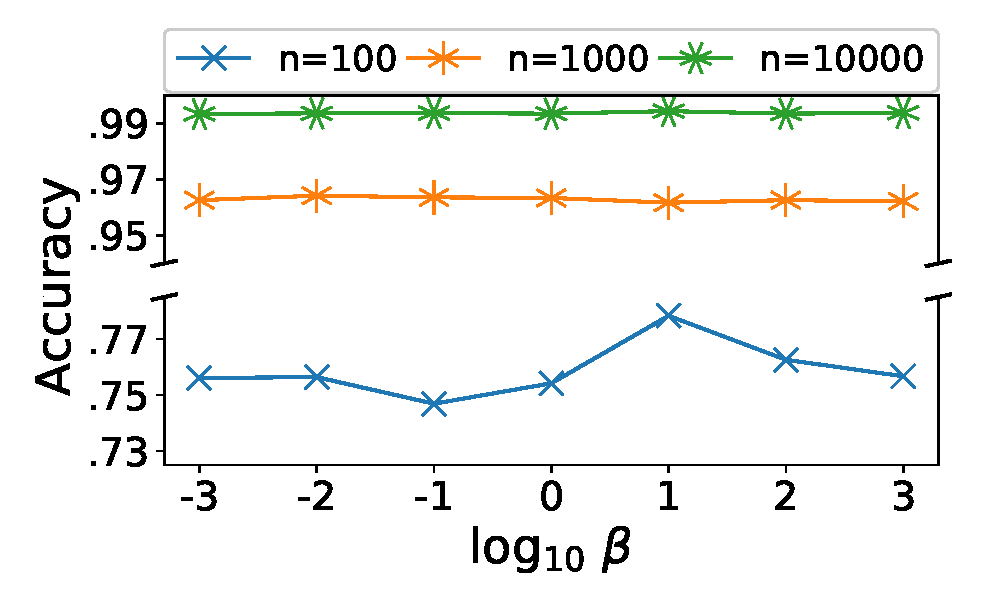
\includegraphics[width=1.00\linewidth]{mdlcompr_mnist_beta.eps}
\end{subfigure}
\hspace*{-0.4em} % \hfill
\begin{subfigure}{0.33\textwidth}
 \centering
 \includegraphics[width=1.00\linewidth]{mdlcompr_mnist_gamma.eps}
\end{subfigure}
\caption{ Effects of hyperparameters in KDGAN on MNIST in the task of model compression.  }
\label{fig:deep model compression tuning}
\end{figure}

We conduct experiments with the tasks of deep model compression and image tag recommendation.
In general, the proposed method can be applied to a wide range of other classification problems where privileged provision is available.
For example, one problem is to classify biopsy images into cancer and non-cancer where historical reports that describe a pathologist's impression about the images are privileged provision.
We experiment with two alternative definitions of the distillation losses, the L2 loss on logits \cite{ba2014deep} and the Kullback–Leibler divergence on distributions \cite{hinton2015distilling}.
The two definitions exhibit comparable results and the results presented in this paper are based on the L2 loss on logits \cite{ba2014deep}.
Since both teacher and discriminator can use privileged provision, we implement the scoring functions $\tchscore$ and $\disscore$ using the same function $\priscore$ with different sets of parameters.
We search the hyperparameters in Equation \ref{equ:objective function} $\alpha$ in $\{0.0,1.0\}$, $\beta$ in $\{0.001,1000\}$, and $\gamma$ in $\{0.0001,100\}$ according to the performance on validation data.
We find that a reasonable schedule for the temperature is to start with a large value and exponentially decay to a small value.
We leave the exploration of the optimal schedule to future work.
In what follows, we test KDGAN, KD-based methods, and the vanilla GAN within the task of deep model compression.
Then, KDGAN is further investigated in the task of image tag recommendation.

\subsection{Deep Model Compression} \label{sec:deep model compression}

The task of deep model compression is to reduce the storage and runtime complexity of deep models and improve the deployability of such models, for example, on mobile devices.
Extensive computing power available for training is considered privileged provision in this task.

\TBF{Experiment Setup}.
We make use of the widely used MNIST \cite{lecun1998gradient} and CIFAR-10 \cite{krizhevsky2009learning} datasets.
The MNIST dataset consists of 10 labels and 60,000 gray images (50,000 for training and 10,000 for testing).
Following \cite{sau2016deep}, we do not preprocess the images on MNIST.
The CIFAR-10 dataset contains 10 labels and 60,000 colored images (50,000 for training and 10,000 for testing).
We preprocess the images by subtracting per-pixel mean and augment the training data by mirrored images.

The scoring functions $\stdscore$ and $\priscore$ are implemented as a MLP \cite{lecun1998gradient} and a LeNet \cite{lecun1998gradient} on MNIST; while as a LeNet \cite{lecun1998gradient} and a ResNet \cite{he2016deep} on CIFAR-10 (detailed in Appendix \ref{app:architecture}).
We compare the proposed KDGAN with KD-based methods and the vanilla GAN in terms of accuracy.
The compared KD-based methods include MIMIC \cite{ba2014deep}, DISTN \cite{hinton2015distilling}, and NOISY \cite{sau2016deep}.
We vary the number of training instances in $\{100,10000\}$ on MNIST and in $\{500,50000\}$ on CIFAR-10.

\TBF{Results and Discussions}.
The overall performance of the compared methods on the two datasets is shown in Table \ref{tab:deep model compression overall}.
From Table \ref{tab:deep model compression overall}, we can see clear performance improvement brought by KDGAN over the baseline methods.
Compared with KD-based methods where the student cannot exceed the pretrained teacher, we find that the student in KDGAN outperforms the pretrained teacher on MNIST.
One possible reason is that KDGAN trains the student, teacher, and discriminator simultaneously in an adversarial way.
The discriminator guides the teacher to generate more realistic labels and achieve better performance.
The improvement of the teacher raises the performance upper bound of the student in theory.
This makes the student have the potential to outperform the pretrained teacher.

Table \ref{tab:deep model compression overall} shows that KDGAN achieves a larger performance gain over the vanilla GAN as the number of training instances decreases.
In other words, KDGAN requires less labeled instances than the vanilla GAN to reach a certain degree of accuracy.
Our explanation is that the teacher provides soft labels which generally have little noise and high entropy.
The soft labels contain much information and serve as more labeled instances to train the student.
Typical learning curves of the student in KDGAN and the vanilla GAN are shown in Figure \ref{fig:learning curves}(a).
Due to page limit, we only show the results using 50,000 training images on CIFAR-10.
We observe that KDGAN converges with less training epochs (about 35 epochs) than the vanilla GAN (about 130 epochs).
Moreover, the student in KDGAN converges to a higher performance with less variance than the vanilla GAN.
% Moreover, we can see that the proposed KDGAN shows an advantage in the low-data regime: KDGAN has a significant lager performance gain over other methods in the cases where we have less labeled training examples.

Figure \ref{fig:deep model compression tuning} shows how the performance of our method varies against the hyperparameters on MNIST.
Note that the log scale of the x axis in Figures \ref{fig:deep model compression tuning}(b) and \ref{fig:deep model compression tuning}(c).
% We achieve similar results on CIFAR-10, which are omitted here due to page limit.
We can see that $\alpha$ and $\beta$ have a relatively small effect on the performance, which suggests that KDGAN is a robust framework.
However, a large value of $\gamma$ causes the performance to deteriorate greatly.
This is because the soft labels provided by the student are quite noisy and contain much errors.
Emphasizing too much on training the teacher to fit the noisy labels decreases the teacher's performance, which in turn decreases the student's performance.
We obtain similar results about the hyperparameter effects on CIFAR-10.

\subsection{Image Tag Recommendation} \label{sec:image tag recommendation}

\begin{figure}[tbp]
\centering
\setlength{\abovecaptionskip}{4pt plus 0pt minus 0pt}
\begin{subfigure}{0.49\textwidth}
 \centering
 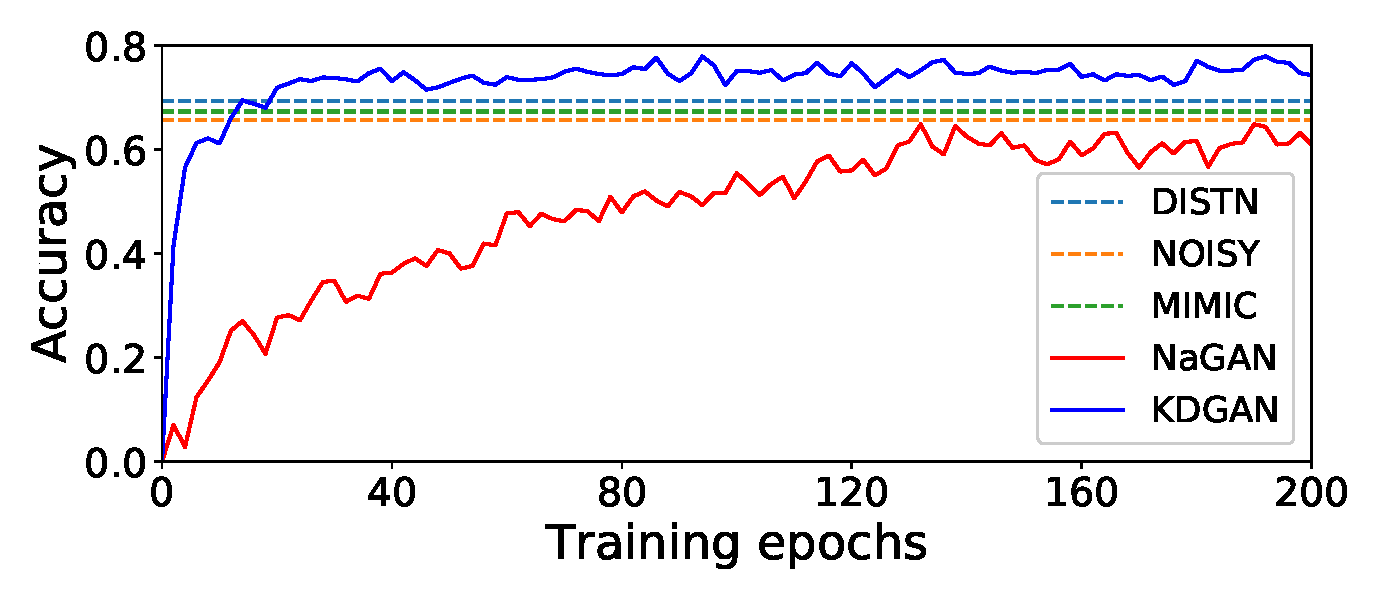
\includegraphics[width=1.00\linewidth]{mdlcompr_mnist_cr.eps}
  \caption{ Deep model compression. }
\end{subfigure}
\begin{subfigure}{0.49\textwidth}
 \centering
 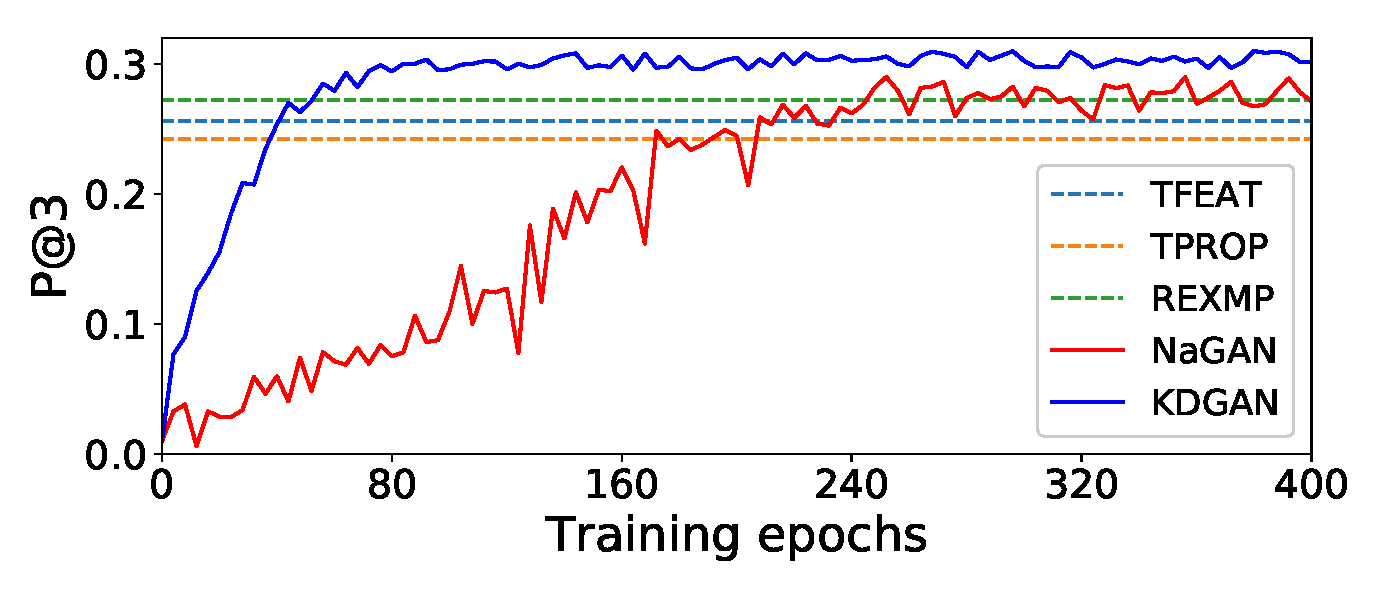
\includegraphics[width=1.00\linewidth]{tagrecom_yfcc10k_cr.eps}
  \caption{ Image tag recommendation. }
\end{subfigure}
\caption{ Learning curves of the proposed KDGAN and a vanilla GAN. }
\label{fig:learning curves}
\end{figure}

Image tag recommendation is to recommend relevant tags (or labels) after a user uploads an image to image-hosting websites such as Instagram\footnote{\url{https://www.instagram.com/}} or Flickr\footnote{\url{https://www.flickr.com/}}.
% For example, if a user uploads an image of a cat playing with a dog, we could recommend relevant tags such as ``cute kitten'', ``lovely pet'', ``brave dog'' etc.
It is common that additional text such as descriptions is provided by the user during uploading the image.
Since text entering is not convenient especially on mobile devices, for better user experience, we aim to make recommendations after a user uploading an image before entering any text.
Hence, we consider the additional text as privileged information in the task of image tag recommendation.


\TBF{Experiment Setup}.
We use the Yahoo Flickr Creative Commons 100 Million (YFCC100M) dataset \cite{thomee2016yfcc100m}.
To simulate the case where additional text about images is available for training, we randomly sample 20,000 images with additional text as the training data and another 2,000 images as the testing data.
We create two datasets with different characteristics, one dataset is annotated with the 200 most popular labels and the other dataset is annotated with 200 randomly sampled labels.

Following existing work \cite{antol2015vqa}, we use a VGGNet \cite{simonyan2014very} pretrained on ImageNet \cite{deng2009imagenet} to extract image features and a LSTM \cite{hochreiter1997long} with pretrained word embeddings \cite{mikolov2013distributed} to learn text features.
We implement $\stdscore$ as a MLP with image features as inputs and $\priscore$ as a MLP with the element-wise product of image and text features as inputs.
The network architectures are detailed in Appendix \ref{app:architecture}.

In experiments, we compare the student in KDGAN with KNN \cite{makadia2010baselines}, TPROP \cite{guillaumin2009tagprop}, TFEAT \cite{chen2012tag}, and REXMP \cite{li2013classifying}.
We use standard ranking measures including precision (P@N), F-score (F@N), mean average precision (MAP), and mean reciprocal ranking (MRR).

\TBF{Results and Discussions}.
The overall results are presented in Table \ref{tab:image tag recommendation overall}.
We observe that KDGAN achieves statistically significant improvements over the other methods across all the measures.
Although KDGAN does not explicitly learn to model the semantic similarity between two labels like what REXMP does, it still works better than REXMP.
A possible explanation is that the teacher provides the student with soft labels during training.
The soft labels contain a rich similarity structure over labels which cannot be modeled well by any pairwise similarity between labels used in REXMP.
For example, an image labeled with volleyball is supplied with a soft label assigning a probability of 10$^{-2}$ to basketball, 10$^{-4}$ to baseball, and 10$^{-8}$ to dragonfly.
How the teacher generalizes is reflected in the relative probabilities of incorrect labels, which trains the student to generalize better.

We further investigate the training curves of KDGAN and the vanilla GAN.
We only show the performance measured by P@3 in Figure \ref{fig:learning curves}(b) and the other measures show similar training curves.
From Figure \ref{fig:learning curves}(b), we find that KDGAN converges to a better equilibrium with less training epochs (about 100 epochs) than the vanilla GAN (about 220 epochs).
After convergence, KDGAN consistently outperforms the best baseline method REXMP.

We also investigate how the performance of the proposed method varies against the hyperparameters on the YFCC100M dataset with the 200 most popular labels.
The results are shown in Figure \ref{fig:image tag recommendation tuning}, which are consistent with our observations in the task of deep model compression.


\section{Conclusion}

\begin{table} [tbp]
\small
\centering
\setlength{\abovecaptionskip}{6pt plus 0pt minus 0pt}
\setlength\tabcolsep{4.5pt}
% \begin{tabular}{l|cccccc|cccccc}
\begin{tabular}{l|C{0.72cm}C{0.72cm}C{0.72cm}C{0.72cm}C{0.72cm}C{0.72cm}|C{0.72cm}C{0.72cm}C{0.72cm}C{0.72cm}C{0.72cm}C{0.72cm}}
\toprule
\multirow{2}{*}{Method} & \multicolumn{6}{c|}{ Popular Labels } & \multicolumn{6}{c}{ Random Labels } \\
\cmidrule(rl){2-7}
\cmidrule(rl){8-13}
& P@3 & P@5 & F@3 & F@5 & MAP & MRR & P@3 & P@5 & F@3 & F@5 & MAP & MRR \\
\midrule
KNN & .2320 & .1680 & .2339 & .1633 & .5755 & .5852 & .1623 & .1198 & .1575 & .1088 & .3970 & .4092 \\
TPROP & .2420 & .1636 & .2811 & .1949 & .6177 & .6270 & .1883 & .1372 & .1810 & .1252 & .4512 & .4636 \\
TFEAT & .2560 & .1752 & .2871 & .1999 & .6417 & .6503 & .2002 & .1420 & .2195 & .1495 & .5149 & .5309 \\
REXMP & .2720 & .1800 & .3324 & .2295 & .7015 & .7122 & .2228 & .1378 & .2427 & .1669 & .5205 & .5331  \\
\midrule
KDGAN & \TBF{.3047} & \TBF{.1968} & \TBF{.3678} & \TBF{.2526} & \TBF{.7787} & \TBF{.7905} & \TBF{.2572} & \TBF{.1666} & \TBF{.2946} & \TBF{.2009} & \TBF{.6302} & \TBF{.6452} \\
\bottomrule
\end{tabular}
\caption{ Performance of various methods on the YFCC100M dataset in tag recommendation.  }
\label{tab:image tag recommendation overall}
\end{table}

\begin{figure}[tbp]
\centering
\setlength{\abovecaptionskip}{4pt plus 0pt minus 0pt}
\begin{subfigure}{.33\textwidth}
 \centering
 \includegraphics[width=1\linewidth]{tagrecom_yfcc10k_alpha.eps}
\end{subfigure}
\hspace*{-0.4em} % \hfill
\begin{subfigure}{.33\textwidth}
 \centering
 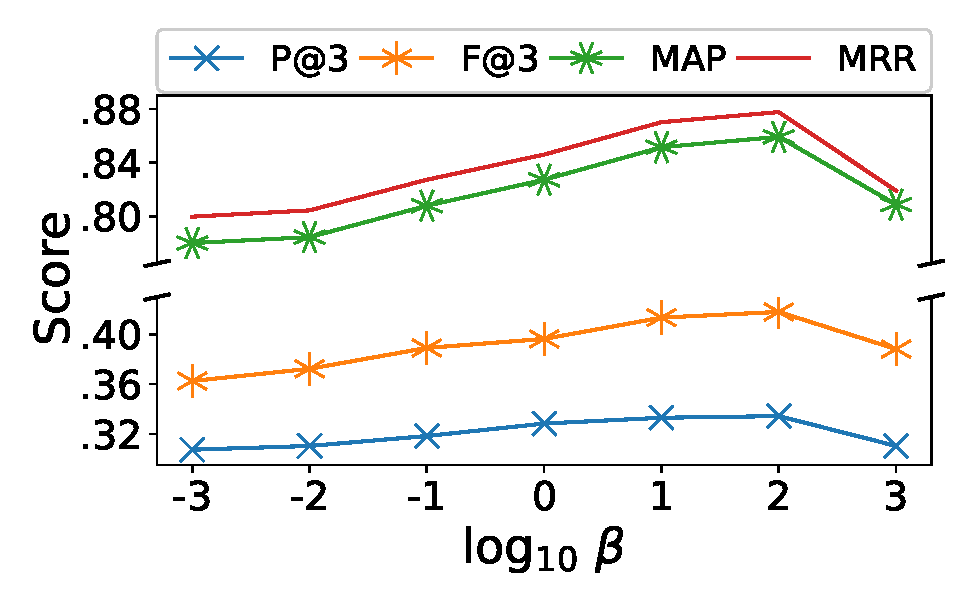
\includegraphics[width=1\linewidth]{tagrecom_yfcc10k_beta.eps}
\end{subfigure}
\hspace*{-0.4em} % \hfill
\begin{subfigure}{.33\textwidth}
 \centering
 \includegraphics[width=1\linewidth]{tagrecom_yfcc10k_gamma.eps}
\end{subfigure}
\caption{ Effects of hyperparameters in KDGAN on YFCC100M in the task of tag recommendation. }
\label{fig:image tag recommendation tuning}
\end{figure}

Motivated by our observations that the advantages and disadvantages of knowledge distillation (KD) and generative adversarial networks (GAN) are complementary, we proposed to power knowledge distillation with generative adversarial networks (KDGAN).
To perform the learning with privileged provision, we formulated KDGAN as a minimax game with a student, a teacher and a discriminator.
With the constraints imposed by the distillation losses and the adversarial losses, KDGAN guarantees that the student perfectly fits the data distribution at the equilibrium.
We showed that integrating KD into GAN accelerates the training by reducing the variance of gradients.
To further reduce the gradient variance, we relaxed the discrete variances used to estimate the gradients into continuous variances with the concrete distribution.
We applied KDGAN to the tasks of image tag recommendation and deep model compression on several widely used datasets.
The experiments showed that KDGAN outperforms several state-of-the-art methods by a quite large margin (e.g., as much as 12.02\% under P@3 in the task of image tag recommendation).
The experiments also showed that the student in KDGAN learns faster and converge to a better equilibrium than the vanilla GAN.


% \clearpage
{
\scriptsize
% \bibliographystyle{unsrtnat}
\bibliographystyle{abbrvnat}
\bibliography{nips_2018}
}


\appendix


\section{Theoretical Analysis} \label{app:theory}

% We provide detailed theoretical analysis of KDGAN in this section.
% Formally, we provide some theoretical results about KDGAN.
We first show that the optimal discriminator balances between the data distribution and the mixture distribution, as stated below.
\begin{corollary1}
For any fixed student and teacher, the objective function $\kdganfullobj$ is maximized if and only if the discriminator $\fullpdis{\OVEC{y}}=\nicefrac{\fullpdat}{(\fullpdat+\fullpmix)}$.
\end{corollary1}%
\begin{proof}
The discriminator aims to maximize the objective function of the minimax game.
According to the definition of the expected value, the objective function can be rewritten as:
\begin{small}
\begin{equation*}
\begin{aligned}
\max_{d}
&
\,
\kdganfullobj
\\
=
&
\,
% \max_{d}
% \big(
\EXP_{\OVEC{y}\sim\abbrpdat}[\log\fullpdis{\OVEC{y}}]
+
\alpha\EXP_{\OVEC{y}\sim\abbrpstd}[\log(1-\fullpdis{\OVEC{y}})]
+
(1-\alpha)\EXP_{\OVEC{y}\sim\abbrptch}[\log(1-\fullpdis{\OVEC{y}})]
% \big)
\\
=
&
\,
% \max_{d}
% \big(
\EXP_{\OVEC{y}\sim\abbrpdat}[\log\fullpdis{\OVEC{y}}]
+
\alpha\sum_{\OVEC{y}}
\fullpstd{\OVEC{y}}\log(1-\fullpdis{\OVEC{y}})
+
(1-\alpha)\sum_{\OVEC{y}}
\fullptch{\OVEC{y}}\log(1-\fullpdis{\OVEC{y}})
% \big)
\\
=
&
\,
% \max_{d}
% \big(
\EXP_{\OVEC{y}\sim\abbrpdat}[\log\fullpdis{\OVEC{y}}]
+
\sum_{\OVEC{y}}
\big(\alpha\fullpstd{\OVEC{y}}+(1-\alpha)\fullptch{\OVEC{y}}\big)
\log(1-\fullpdis{\OVEC{y}})
% \big)
\\
=
&
\,
% \max_{d}
% \big(
\EXP_{\OVEC{y}\sim\abbrpdat}[\log\fullpdis{\OVEC{y}}]
+
\sum_{\OVEC{y}}
\fullpmix\log(1-\fullpdis{\OVEC{y}})
% \big)
\\
=
&
% \max_{d}
% \big(
\sum_{\OVEC{y}}
\fullpdat\log\fullpdis{\OVEC{y}}
+
\sum_{\OVEC{y}}
\fullpmix\log(1-\fullpdis{\OVEC{y}})
% \big)
\text{,}
\end{aligned}
\end{equation*}%
\end{small}%
which reaches the maximum at $\fullpdis{\OVEC{y}}=\nicefrac{\fullpdat}{\fullpdat+\fullpmix}$, concluding the proof.
\end{proof}
Further, we show that the equilibrium of the minimax game is achieved iff both the student and teacher are exactly the same as the data distribution, which is summarized as follows.
\begin{theorem1}
The equilibrium of the minimax game $\kdganmin\kdganmax\kdganfullobj$ is achieved if and only if $\fullpstd{\OVEC{y}}=\fullptch{\OVEC{y}}=\fullpdat$. At that point, $\kdganfullobj$ reaches the value $-\log 4$.
\end{theorem1}%
\begin{proof}
We decompose the value function $\kdganfullobj$ into $\kdgandistillation$ consisting of the distillation losses and $\kdganadversarial$ consisting of the adversarial losses:
\begin{small}
\begin{equation*}
\begin{aligned}
\kdgandistillation
&=
\beta\stddistloss(\fullpstd{\OVEC{y}},\fullptch{\OVEC{y}})
+
\gamma\tchdistloss(\fullptch{\OVEC{y}},\fullpstd{\OVEC{y}})
\\
\kdganadversarial
&=
\EXP_{\OVEC{y}\sim\abbrpdat}[\log\fullpdis{\OVEC{y}}]
+
\alpha\EXP_{\OVEC{y}\sim\abbrpstd}[\log(1-\fullpdis{\OVEC{y}})]
+
(1-\alpha)\EXP_{\OVEC{y}\sim\abbrptch}[\log(1-\fullpdis{\OVEC{y}})]
\\
\end{aligned}
\end{equation*}
\end{small}%
Given the optimal discriminator, we minimize the value function $\kdganfullobj$ as:
\begin{small}
\begin{equation*}
\begin{aligned}
\min_{s,t}
&
\,
\kdganfullobj
\\
=
&
\sum_{\OVEC{y}}
\fullpdat\log\frac{\fullpdat}{\fullpdat+\fullpmix}
+
\sum_{\OVEC{y}}
\fullpmix\log(1-\frac{\fullpdat}{\fullpdat+\fullpmix})
+
\kdgandistillation
\\
=
&
\sum_{\OVEC{y}}
\fullpdat\log\frac{\fullpdat}{\fullpdat+\fullpmix}
+
\sum_{\OVEC{y}}
\fullpmix\log\frac{\fullpmix}{\fullpdat+\fullpmix}
+
\kdgandistillation
\\
=
&
-\log(4)
+
\LOSS{L}{KL}(\fullpdat||\frac{\fullpdat+\fullpmix}{2})
+
\LOSS{L}{KL}(\fullpmix||\frac{\fullpdat+\fullpmix}{2})
+
\kdgandistillation
\\
=
&
-\log(4)
+
\LOSS{L}{JS}(\fullpdat||\fullpmix)
+
\beta\stddistloss(\fullpstd{\OVEC{y}},\fullptch{\OVEC{y}})
+
\gamma\tchdistloss(\fullptch{\OVEC{y}},\fullpstd{\OVEC{y}})
\\
\end{aligned}
\end{equation*}%
\end{small}%
Here, $\LOSS{L}{KL}$ is the Kullback–Leibler divergence and $\LOSS{L}{JS}$ is the Jensen-Shannon divergence which is always non-negative and reaches zero if and only if $\fullpdat=\fullpmix$.
The distillation losses $\stddistloss$ and $\tchdistloss$ such as the L2 loss and the Kullback–Leibler divergence achieve the minimum at zero if and only if $\fullpstd{\OVEC{y}}=\fullptch{\OVEC{y}}$.
Therefore, the value function reaches the minimum at $-\log 4$ if and only if $\fullpstd{\OVEC{y}}=\fullptch{\OVEC{y}}=\fullpmix=\fullpdat$, which concludes the proof.
\end{proof}

\begin{lemma1}
Let $X$ and $Y$ be two random variables that satisfy $\VAR(X)\geq\VAR(Y)$.
Then for all $\lambda\in\interval{0}{1}$, we have $\VAR(X)\geq\VAR(Z)$ where $Z = \lambda X+ (1-\lambda) Y$.
\end{lemma1}
 
\begin{proof}
Given $\VAR(X)\geq\VAR(Y)$, the covariance $\COV(X,Y)$ is upper bounded by $\VAR(X)$.
% \begin{small}
\begin{equation}
\begin{aligned}
\COV(X,Y)
\leq
|\COV(X,Y)|
\leq
\sqrt{\VAR(X)\VAR(Y)}
\leq
\sqrt{\VAR(X)\VAR(X)}
\leq
\VAR(X)
\end{aligned}
\end{equation}%
% \end{small}%
According to the properties of the variance, we have
% \begin{small}
\begin{equation}
\begin{aligned}
\VAR(Z)
=
&
\lambda^{2}\VAR(X)
+
(1-\lambda)^{2}\VAR(Y)
+
2\lambda(1-\lambda)\COV(X,Y)
\\
\leq
&
\lambda^{2}\VAR(X)
+
(1-\lambda)^{2}\VAR(X)
+
2\lambda(1-\lambda)\COV(X,Y)
\\
\leq
&
\lambda^{2}\VAR(X)
+
(1-\lambda)^{2}\VAR(X)
+
2\lambda(1-\lambda)\VAR(X)
=
\VAR(X)
\text{,}
\end{aligned}
\end{equation}%
% \end{small}%
which concludes the proof.
\end{proof}


\section{Gradient Derivation} \label{app:gradient}

We provide the detailed derivation for the gradients of the value function in the KDGAN framework.
Similar to the definition of the concrete distribution $\fullqstd{\OVEC{y}}$ for the student in Equation \ref{equ:student concrete distribution}, the concrete distribution $\fullqtch{\OVEC{y}}$ for the teacher is defined as:
\begin{small}
\begin{equation*} \label{equ:teacher concrete distribution}
\begin{aligned}
\fullqtch{\OVEC{y}}
=
\text{softmax}(\frac{\log\fullptch{\OVEC{y}}+\OVEC{g}}{\tau})
\text{, }
\quad
\OVEC{g}=-\log(-\log(\OVEC{u}))
\text{, }
\quad
\OVEC{u}\sim\text{uniform}\interval[open left, open right]{0}{1}
\text{,}
\end{aligned}
\end{equation*}
\end{small}%
where $\tau\in\interval[open left, open right]{0}{+\infty}$ is a temperature.
The student and teacher generate pseudo labels by sampling from the concrete distributions $\fullqstd{\OVEC{y}}$ and $\fullqtch{\OVEC{y}}$.
Given the pseudo labels and the true labels for a training example, the discriminator aims to maximize the probability of correctly identifying the true labels as positive and the pseudo labels as negative.
The discriminator is trained by maximizing the value function $\kdganfullobj$ as follows:
\begin{small}
\begin{equation*}
\begin{aligned}
\nabla_{d}
\kdganabbrobj
=
&
\nabla_{d}
\big(
\EXP_{\OVEC{y}\sim\abbrpdat}[\log\fullpdis{\OVEC{y}}]
+
\alpha
\EXP_{\OVEC{y}\sim\abbrpstd}[\log(1-\fullpdis{\OVEC{y}})]
+
(1 - \alpha)
\EXP_{\OVEC{y}\sim\abbrptch}[\log(1-\fullpdis{\OVEC{y}})]
\big)
\\
\approx
&
\nabla_{d}
\big(
\EXP_{\OVEC{y}\sim\abbrpdat}[\log\fullpdis{\OVEC{y}}]
+
\alpha
\EXP_{\OVEC{y}\sim\abbrqstd}[\log(1-\fullpdis{\OVEC{y}})]
+
(1 - \alpha)
\EXP_{\OVEC{y}\sim\abbrqtch}[\log(1-\fullpdis{\OVEC{y}})]
\big)
\\
\approx
&
{\textstyle\frac{1}{k}}
{\textstyle\sum}_{i=1}^{k}
\big(
\nabla_{d}
\log\fullpdis{\OVEC{y}_{i}}
+
\alpha\nabla_{d}\log(1-\fullpdis{\SVEC{y}^{i}_{s}})
+
(1-\alpha)\nabla_{d}\log(1-\fullpdis{\SVEC{y}^{i}_{t}})
\big)
\\
\end{aligned}
\end{equation*}
\end{small}%
Here, $k$ is the number of samples used to estimate the gradient.
Labels $y_{i}$, $\SVEC{y}^{i}_{s}$, and $\SVEC{y}^{i}_{t}$ are sampled from $\fullpdat$, $\fullqstd{\OVEC{y}}$, and $\fullqtch{\OVEC{y}}$ respectively.

By contrast, the student aims to generate the pseudo labels that look like the true labels as well as the soft labels produced by the teacher by minimizing the value function as:
\begin{small}
\begin{equation*}
\begin{aligned}
\nabla_{s}
\kdganabbrobj
&=
\nabla_{s}
\big(
\alpha\EXP_{\OVEC{y}\sim\abbrpstd}[\log(1-\fullpdis{\OVEC{y}})]
+
\beta\stddistloss(\fullpstd{\OVEC{y}},\fullptch{\OVEC{y}})
\big)
\\
&=
\alpha{\textstyle\sum}_{\OVEC{y}}
\nabla_{s}\fullpstd{\OVEC{y}}\log(1-\fullpdis{\OVEC{y}})
+
\beta\nabla_{s}\stddistloss(\fullpstd{\OVEC{y}},\fullptch{\OVEC{y}})
\\
&=
\alpha{\textstyle\sum}_{\OVEC{y}}
\fullpstd{\OVEC{y}}\nabla_{s}\log\fullpstd{\OVEC{y}}\log(1-\fullpdis{\OVEC{y}})
+
\beta\nabla_{s}\stddistloss(\fullpstd{\OVEC{y}},\fullptch{\OVEC{y}})
\\
&=
\alpha\EXP_{\OVEC{y}\sim\abbrpstd}
[\nabla_{s}\log\fullpstd{\OVEC{y}}\log(1-\fullpdis{\OVEC{y}})]
+
\beta\nabla_{s}\stddistloss(\fullpstd{\OVEC{y}},\fullptch{\OVEC{y}})
\\
&\approx
\alpha\EXP_{\OVEC{y}\sim\abbrqstd}
[\nabla_{s}\log\fullqstd{\OVEC{y}}\log(1-\fullpdis{\OVEC{y}})]
+
\beta\nabla_{s}\stddistloss(\fullpstd{\OVEC{y}},\fullptch{\OVEC{y}})
\\
&\approx
{\textstyle\frac{1}{k}}
{\textstyle\sum}_{i=1}^{k}
\alpha
\nabla_{s}\log\fullqstd{\OVEC{y}^{i}_{s}}
\log(1-\fullpdis{\SVEC{y}^{i}_{s}})
+
\beta
\nabla_{s}
\stddistloss(\fullpstd{\OVEC{y}},\fullptch{\OVEC{y}})
\text{,}
\\
\end{aligned}
\end{equation*}
\end{small}%
where $\SVEC{y}^{i}_{s}$ a one-hot label that encodes the argument of the maxima for a sampled from $\fullqstd{\OVEC{y}}$.
To further reduce the gradient variance during training, we use a control variate defined as \cite{wang2017irgan}
% \begin{small}
\begin{equation} \label{equ:baseline function}
\begin{aligned}
b_{s}
=
\EXP_{\OVEC{y}\sim\fullqstd{\OVEC{y}}}
[\log(1-\fullpdis{\OVEC{y}})]
=
{\textstyle\sum}_{i=1}^{k}\log(1-\fullpdis{\SVEC{y}^{i}_{s}})
\text{,}
\end{aligned}
\end{equation}%
% \end{small}%
where $\SVEC{y}_{s}$ is sampled from the concrete distribution $\fullqstd{\OVEC{y}}$.
$\nabla_{s}\stddistloss$ is the gradients of the distillation loss $\stddistloss$, which can be easily computed by the back-propagation algorithm.
For example, if we define the distillation loss as the L2 loss \cite{ba2014deep}, the gradients are computed by
\begin{small}
\begin{equation*}
\begin{aligned}
\nabla_{s}
\stddistloss(\fullpstd{\OVEC{y}},\fullptch{\OVEC{y}})
=
-
||\log\fullptch{\OVEC{y}}-\log\fullpstd{\OVEC{y}})||
\nabla_{s}\log\fullpstd{\OVEC{y}}
\\
\end{aligned}
\end{equation*}
\end{small}%
Similarly, the gradients to update the teacher are derived as follows,
\begin{small}
\begin{equation*}
\begin{aligned}
\nabla_{t}
\kdganabbrobj
&=
\nabla_{t}
\big(
(1-\alpha)\EXP_{\OVEC{y}\sim\abbrptch}[\log(1-\fullpdis{\OVEC{y}})]
+
\gamma\tchdistloss(\fullptch{\OVEC{y}},\fullpstd{\OVEC{y}})
\big)
\\
&=
(1-\alpha){\textstyle\sum}_{\OVEC{y}}
\nabla_{t}\fullptch{\OVEC{y}}\log(1-\fullpdis{\OVEC{y}})
+
\gamma\nabla_{t}\tchdistloss(\fullptch{\OVEC{y}},\fullpstd{\OVEC{y}})
\\
&=
(1-\alpha){\textstyle\sum}_{\OVEC{y}}
\fullptch{\OVEC{y}}\nabla_{t}\log\fullptch{\OVEC{y}}\log(1-\fullpdis{\OVEC{y}})
+
\gamma\nabla_{t}\tchdistloss(\fullptch{\OVEC{y}},\fullpstd{\OVEC{y}})
\\
&=
(1-\alpha)\EXP_{\OVEC{y}\sim\abbrptch}
[\nabla_{t}\log\fullptch{\OVEC{y}}\log(1-\fullpdis{\OVEC{y}})]
+
\gamma\nabla_{t}\tchdistloss(\fullptch{\OVEC{y}},\fullpstd{\OVEC{y}})
\\
&\approx
(1-\alpha)\EXP_{\OVEC{y}\sim\abbrqtch}
[\nabla_{t}\log\fullqtch{\OVEC{y}}\log(1-\fullpdis{\OVEC{y}})]
+
\gamma\nabla_{t}\tchdistloss(\fullptch{\OVEC{y}},\fullpstd{\OVEC{y}})
\\
&\approx
{\textstyle\frac{1}{k}}
{\textstyle\sum}_{i=1}^{k}
\big(
(1-\alpha)
\nabla_{t}\log\fullqtch{\OVEC{y}^{i}_{t}}
\log(1-\fullpdis{\SVEC{y}^{i}_{t}})
+
\gamma
\nabla_{t}
\tchdistloss(\fullptch{\OVEC{y}},\fullpstd{\OVEC{y}})
\text{,}
\\
\end{aligned}
\end{equation*}
\end{small}%
where $\SVEC{y}^{i}_{t}$ is a one-hot label that encodes the argument of the maxima for a sample from $\fullqtch{\OVEC{y}}$.
We also use a control variate during the training of the teacher, which is defined as
\begin{small}
\begin{equation*}
b_{t}
=
=
\EXP_{\OVEC{y}\sim\fullqtch{\OVEC{y}}}
[\log(1-\fullpdis{\OVEC{y}})]
=
{\textstyle\sum}_{i=1}^{k}\log(1-\fullpdis{\SVEC{y}^{i}_{t}})
\text{,}
\end{equation*}
\end{small}%
where $\SVEC{y}_{t}$ is sampled from the concrete distribution $\fullqtch{\OVEC{y}}$.
$\nabla_{t}\tchdistloss$ is the gradients of the distillation loss $\tchdistloss$.
For example, $\nabla_{t}\tchdistloss$ is computed by
\begin{small}
\begin{equation*}
\begin{aligned}
\nabla_{t}
\tchdistloss(\fullptch{\OVEC{y}},\fullpstd{\OVEC{y}})
=
-
||\log\fullpstd{\OVEC{y}}-\log\fullptch{\OVEC{y}}||
\nabla_{t}\log\fullptch{\OVEC{y}}
\text{,}
\\
\end{aligned}
\end{equation*}
\end{small}%
when the distillation loss is defined as the L2 loss \cite{ba2014deep}.


\section{Network Architectures} \label{app:architecture}

First, we describe the network architectures in the experiments of deep model compression on the MNIST dataset.
We implement the scoring function $\stdscore$ as a MLP.
The architecture of the MLP is written as
\begin{enumerate}
\item An input layer of a 28$\times$28 gray image.
\item A stack of 2 fully connected layer with 800 neurons.
\item A softmax layer with 10 classes.
\end{enumerate}
We implement the scoring function $\priscore$ as a LeNet.
The architecture of the LeNet is given by
\begin{enumerate}
\item An input layer of a 28$\times$28 gray image.
\item A convolutional layer with 20 kernels of size 5$\times$5 and stride 1.
\item A max pooling layer with size 2$\times$2 and stride 2.
\item A convolutional layer with 20 kernels of size5$\times$5 and stride 1.
\item A max pooling layer with size 2$\times$2 and stride 2.
\item A fully connected layer with 500 neurons.
\item A softmax layer with 10 classes.
\end{enumerate}

Then, we describe the network architectures in the experiments of deep model compression on the CIFAR-10 dataset.
We implement the scoring function $\stdscore$ as a LeNet.
The architecture of the LeNet is written as
\begin{enumerate}
\item An input layer of a 32$\times$32 colored image.
\item A convolutional layer with 64 kernels of size 5$\times$5 and stride 1.
\item A max pooling layer with size 2$\times$2 and stride 2.
\item A convolutional layer with 128 kernels of size 5$\times$5 and stride 1.
\item A max pooling layer with size 2$\times$2 and stride 2.
\item A fully connected layer with 1024 neurons.
\item A softmax layer with 10 classes.
\end{enumerate}
We implement the scoring function $\priscore$ as a ResNet.
The architecture of the ResNet is given by
\begin{enumerate}
\item An input layer of a 32$\times$32 colored image.
\item A convolutional layer with 16 kernels with size 3$\times$3 and stride 1.
\item Five stacked blocks of 2 convolutional layer with 16 kernels of size 3$\times$3 and stride 1.
\item Five stacked blocks of 2 convolutional layer with 32 kernels of size 3$\times$3.
The first convolutional layer is of stride 2 and the following convolutional layers are of stride 1.
\item Five stacked blocks of 2 convolutional layer with 64 kernels of size 3$\times$3.
The first convolutional layer is of stride 2 and the following convolutional layers are of stride 1.
\item A global pooling layer.
\item A softmax layer with 10 classes.
\end{enumerate}

Finally, we describe the network architectures in the experiments of image tag recommendation on the YFCC100M dataset.
We use the same network architectures when experimenting with the 200 most popular labels and 200 randomly sampled labels.
We implement a VGGNet to extract image features.
The architecture of the VGGNet is written as
\begin{enumerate}
\item An input layer of a 224$\times$224 colored image.
\item A stack of 2 convolutional layers with 64 kernels of size 3$\times$3 and stride 1.
\item A max pooling layer with size 2$\times$2 and stride 2.
\item A stack of 2 convolutional layers with 128 kernels of size 3$\times$3 and stride 1.
\item A max pooling layer with size 2$\times$2 and stride 2.
\item A stack of 2 convolutional layers with 256 kernels of size 3$\times$3 and stride 1.
\item A max pooling layer with size 2$\times$2 and stride 2.
\item A stack of 2 convolutional layers with 512 kernels of size 3$\times$3 and stride 1.
\item A max pooling layer with size 2$\times$2 and stride 2.
\item A stack of 2 convolutional layers with 512 kernels of size 3$\times$3 and stride 1.
\item A max pooling layer with size 2$\times$2 and stride 2.
\item A fully connected layer with 4096 neurons.
\item A fully connected layer with 4096 neurons.
\item A fully connected layer with 100 neurons.
\end{enumerate}
We implement a LSTM to extract text features.
The architecture of the LSTM is written as
\begin{small}
\begin{equation*}
\begin{aligned}
\OVEC{f}_{t}=&\,\text{sigmoid}(\MAT{W}_{f}\cdot[\OVEC{h}_{t-1},\OVEC{x}_{t}]+\OVEC{b}_{f})\text{,}\\
\OVEC{i}_{t}=&\,\text{sigmoid}(\MAT{W}_{i}\cdot[\OVEC{h}_{t-1},\OVEC{x}_{t}]+\OVEC{b}_{i})\text{,}\\
\OVEC{o}_{t}=&\,\text{sigmoid}(\MAT{W}_{o}\cdot[\OVEC{h}_{t-1},\OVEC{x}_{t}]+\OVEC{b}_{o})\text{,}\\
\OVEC{s}_{t}=&\,\OVEC{f}_{t}\odot\OVEC{s}_{t-1}+
\OVEC{i}_{t}\odot\tanh(\MAT{W}_{s}\cdot[\OVEC{h}_{t-1},\OVEC{x}_{t}]+\OVEC{b}_{s})\text{,}\\
\OVEC{h}_{t}=&\,\OVEC{o}_{t}\odot\tanh(\OVEC{s}_{t})\text{,}
\end{aligned}
\end{equation*}
\end{small}%
where $[\OVEC{h},\OVEC{x}]$ is the vector concatenation and $\cdot$ is the element-wise product.
We set the hidden size of the LSTM to 100 in experiments.
Let $\OVEC{v}_{x} \in \mathbb{R}^{100}$ be the image features extracted by the VGGNet and $\OVEC{v}_{z} \in \mathbb{R}^{100}$ be the text features extracted by the LSTM.
We implement the scoring function $\stdscore$ as a MLP.
The architecture of the MLP is written as
\begin{enumerate}
\item An input layer of a feature vector with size 100 (i.e. the image features $\OVEC{v}_{x}$).
\item A stack of 2 fully connected layers with 800 neurons.
\item A softmax layer with 200 classes.
\end{enumerate}
We implement the scoring function $\priscore$ as a MLP.
The architecture of the MLP is given by
\begin{enumerate}
\item An input layer of a feature vector with size 100 (i.e. the element-wise product of $\OVEC{v}_{x}$ and $\OVEC{v}_{z}$).
\item A stack of 2 fully connected layers with 1200 neurons.
\item A softmax layer with 200 classes.
\end{enumerate}


\end{document}
